\begin{figure}[H]
    \centering

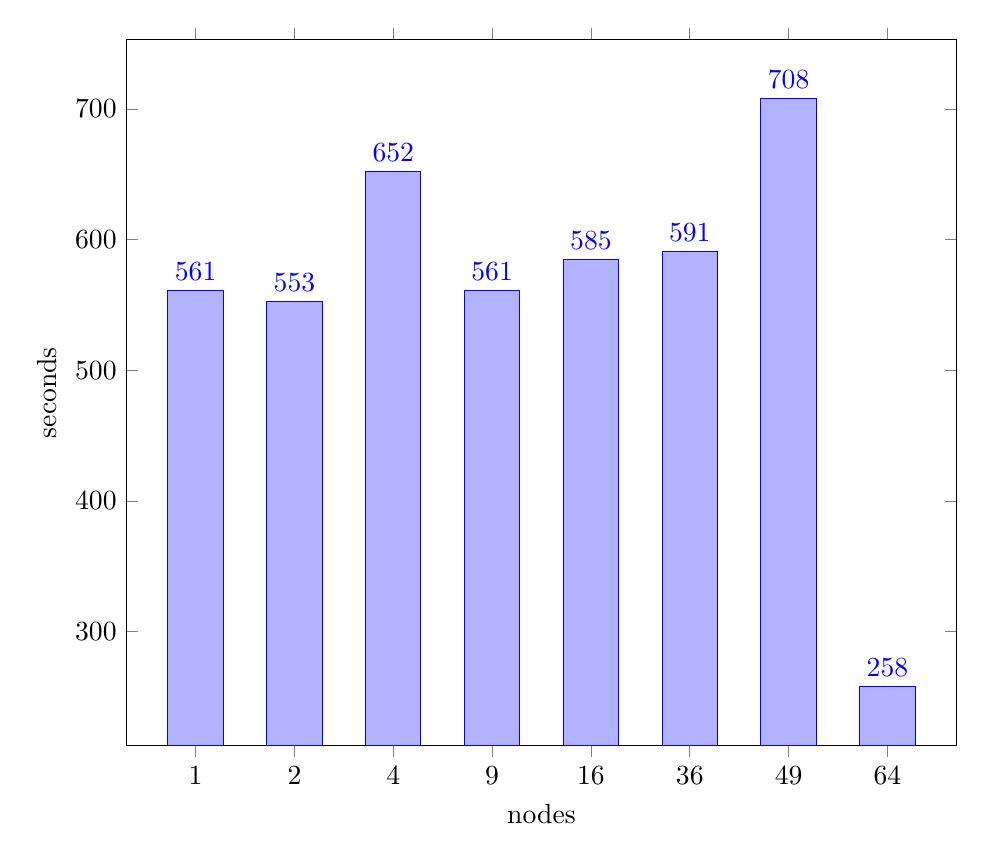
\begin{tikzpicture}
    \begin{axis}[
            ybar,
            enlargelimits=true,
            bar width=20pt,
            width=\textwidth,
            height=300pt,
            legend style={at={(0.5,-0.15)}, anchor=north,legend columns=-1},
            ylabel={seconds},
            xlabel={nodes},
            symbolic x coords={1,2,4,9,16,36,49,64},
            xtick=data,
            nodes near coords,
            nodes near coords align={vertical},
        ]
\addplot coordinates {
(1,561)	% ./guided_new_parser_bin
(2,553)	% ./guided_new_parser_bin
(4,652)	% ./guided_new_parser_bin
(9,561)	% ./guided_new_parser_bin
(16,585)	% ./guided_new_parser_bin
(36,591)	% ./guided_new_parser_bin
(49,708)
(64,258)	% ./guided_new_parser_bin
};
    \end{axis}
\end{tikzpicture}    
\caption{inst1000-80000-20-10-1000}
\label{fig:1000}
\end{figure}